\section{Metodología de desarrollo aplicada a la propuesta} \label{metodologia}
% \section{Metodologías Tradicionales y Metodologías Ágiles}\label{metodologia}
En el marco de las asignaturas Análisis y Diseño de Sistemas e Ingeniería de Software, ambas del tercer año de las carreras Analista, Profesorado y 
 Licenciatura en Ciencias de la Computación de la U.N.R.C, se presentan diferentes metodologías para el desarrollo de 
sistemas informáticos. Algunos de los ciclos de vida del software estudiados son:  el ciclo de vida lineal o secuencial, el método del análisis estructurado de Jourdon\cite{}
, desarrollo basado en componentes, diseño por contratos\cite{} de Bertrand Meyer, el Proceso Unificado \cite{} y metodologías ágiles.\\ 
 
La asignatura Análisis y Diseño de Sistemas cuenta con una planificación de 180 horas.Com se explicó en la sección FUNDAMENTOS, 
en trabajos ateriores se propuso
integrar este proyecto a los proyectos de fin de materia de todas las asignaturas de 3er. año. En esta oportunidad lo que se presenta es
una modificación a este proyecto-taller meditante la incorporación de un set de herramientas 
que la industria de desarrollo de software utiliza actualmente. Dichas tecnologías están intimamente ligadas a la aplicación de metodologías ágiles. 
Es por ello que el cuerpo docente de la asignatura ha seleccionado la metodología ágil SCRUM  CITA  la cual se explcia brevemente en el siguiente apartado.

\subsection{Scrum}
Scrum es una metodología ágil que permite trabajar en ambientes muy cambiantes, permitiendo permanentes replanteamientos. 
Por otro lado permite reducir el tiempo de producción y de comercialización del producto obtenido, aporta un gran beneficio o 
valor agregado al cliente, minimiza los riesgos de desperdiciar esfuerzo/tiempo en la construcción de artefactos que no serán usados 
o que no son fundamentales para el cliente. Facilita también la comunicación entre todos los integrantes del proyecto. 
La documentación producida dentro de un proyecto SCRUM es relativa al usuario, dueño, producto y equipo.  Scrum es más bien un marco de 
trabajo que reposa sobre la premisa de que el equipo de desarrollo conocerá la mejor manera de resolver el problema que se le presenta. 
La reunión de planificación de cada grupo de requerimientos a producir se describe en términos del resultado deseado, 
en lugar de un conjunto de criterios de ingreso, definiciones y tareas. 
Scrum se basa en una auto-organización, con un equipo multifuncional y sin líder (dentro del equipo). 
El equipo es apoyado por dos individuos quienes ocupan los roles de Scrum Master y  Product Owner. 
El Scrum Master es una especie de entrenador para el equipo, su función es ayudar a los miembros del mismo a utilizar el marco que ofrece 
la metodología para conseguir un nivel alto de productividad. Mientras que el Product Owner representa los negocios, clientes o 
usuarios. Éste guía al equipo hacia la construcción del producto adecuado.
 Los proyectos Scrum avanzan en orden a la definición de los sprints, que son las iteraciones que poseen una duración de entre dos y cuatro semanas. 
En el inicio de cada sprint, los miembros del equipo se comprometen a producir un cierto número de características que enumeran en 
el artefacto conocido como el Product Backlog del proyecto.  Al final de cada sprint, cada funcionalidad (conocida como \emph{historia}) debe estar codificada,
 probada e integrada a una versión demo del sprint anterior. Luego se realiza una revisión, y por último se demuestra la nueva funcionalidad
 frente al Product Owner y las otras partes interesadas que proporcionen información requerida para el siguiente sprint. 
Las iteraciones han de continuar hasta obtener el producto deseado.
Como se puede observar de lo expuesto, SCRUM establece una forma de trabajo en donde todo el equipo se auto-regula y en donde no hay de antemano
una documentación establecida a priori. Cada equipo utilizará los elementos que le sean necesarios  para poder llevar adelante el grupo de \emph{historias}
con el cual se ha comprometido. Algunos podrán utilizar diagramas UML\cite{} otros utilizarán diagramas de flujos de datos, etc.
En la figura \ref{figu1} se esquematiza todo el proceso.

\begin{figure}
  \centering
    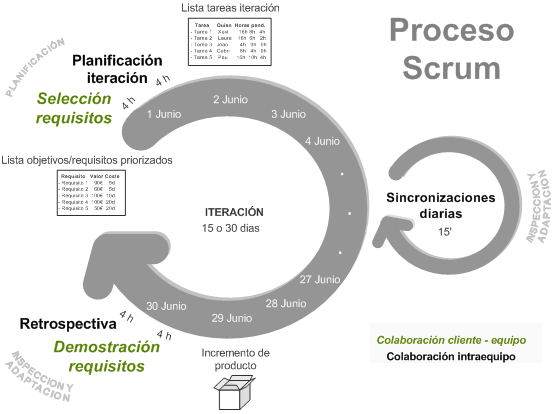
\includegraphics[width=0.85\textwidth]{f2.png}
  \caption{Proceso Scrum}
  \label{figu1}
\end{figure}